\section{PDEs in rectangular coordinates}

In this section, we will consider separation of variable for more general equation in rectangular coordinates, possibly with variable coefficients and more general boundary conditions. 

\subsection{Boundary conditions for general PDEs}


\subsubsection{Dirichlet, Neumann and Robin boundary conditions}

In the ODE class, we have learned the following boundary value problem
\begin{equation}\label{eq.ODE_boundary}
    \begin{split}
        &u'' = 1, \qquad x\in [0, 1]
        \\
        &u(0) = 0,\quad u(1) = 0.
    \end{split}
\end{equation}
where we prescribe a condition for every point on the boundary of the domain $[0, 1]$. (The boundary is $0$ and $1$.) If we missing any of these conditions, we cannot get a unique solution. 

For example, if we remove the condition $u(1) = 0$, then we get solution $u(x) = \frac{1}{2}x^2 + Cx$, which contains an undetermined constant $C$.

Given a PDE defined on a domain $R$, we must also prescibe the boundary condition on $\partial R$ to obtain a unique solution.

\begin{figure}[H]
    \begin{tikzpicture}
        \node at (0, 0) {
            \scalebox{0.2}{      
                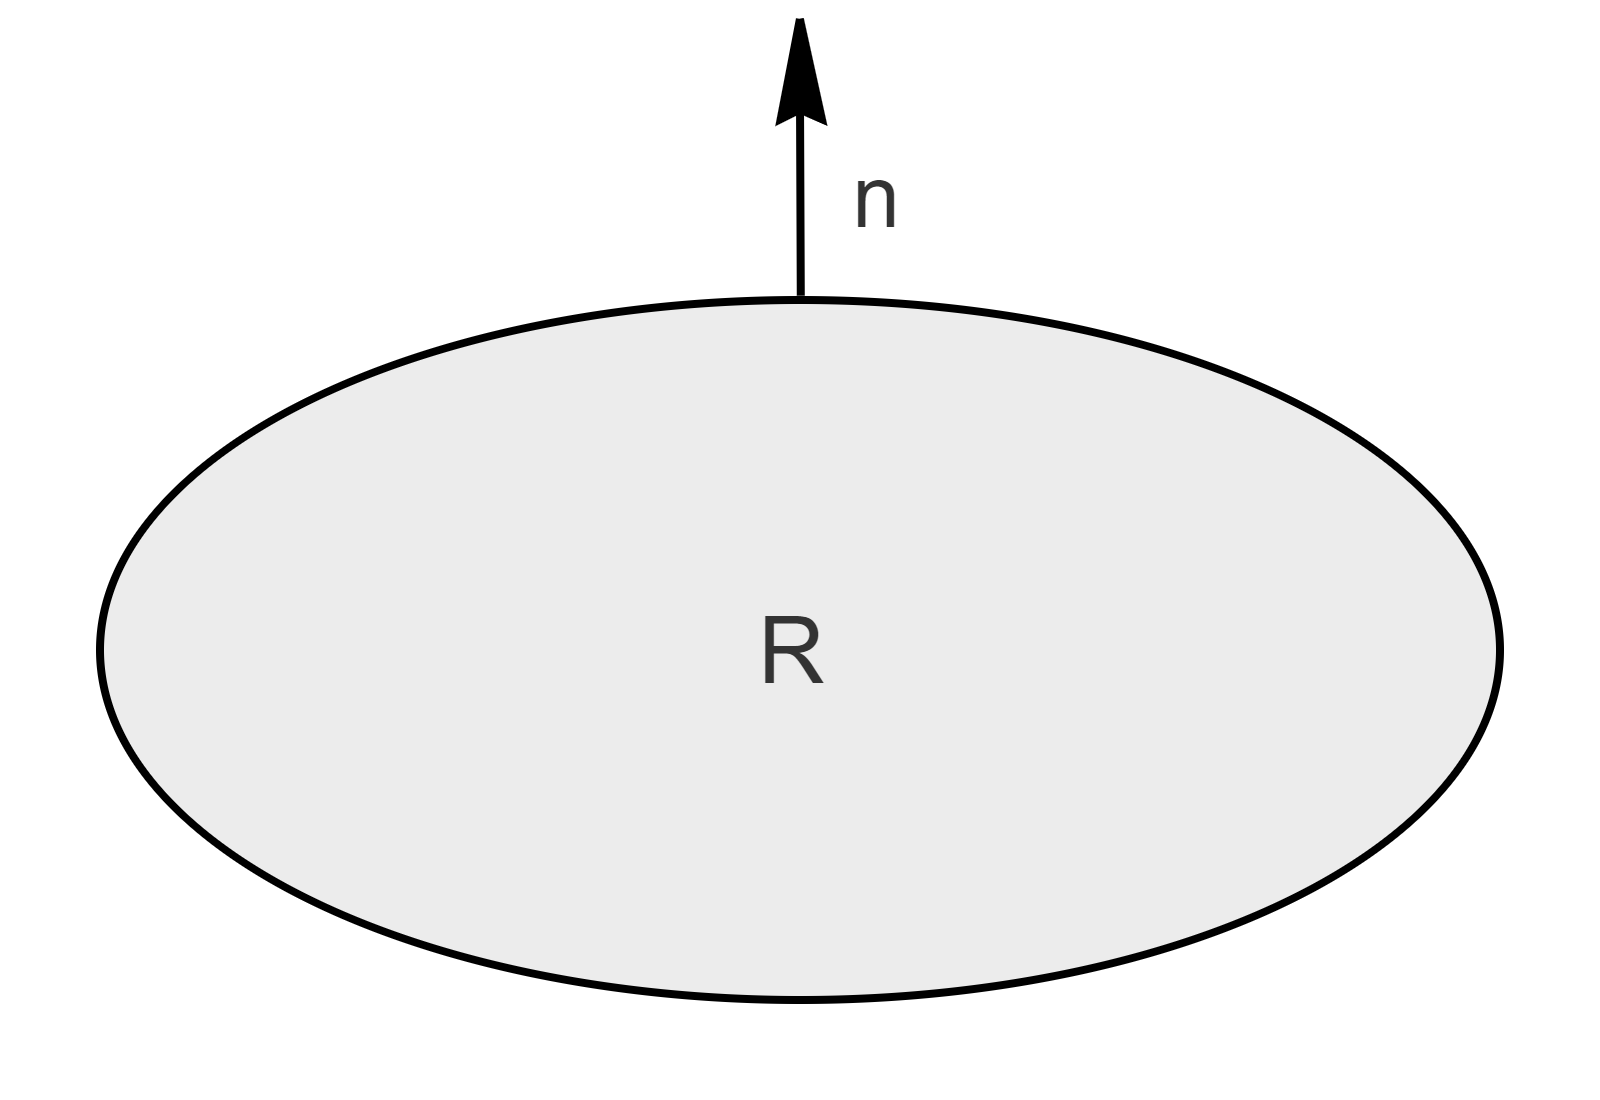
\includegraphics{pictures/normal_vector.png}
            }
        };
        \node at (0.4, 1.8) {$\mathbf{n}$};
        \node at (0, -0.5) {$R$};
    \end{tikzpicture}
    \centering 
    \caption{The region $R$ and its normal vector.} 
    \label{fig.normal_vector} 
\end{figure}

Before we introduce the concept of boundary conditions, let us first explain the concept of normal vectors.

\begin{definition}[Normal vector] Given a domain $R$ and a point $x\in \partial R$, a \underline{normal vector} $\mathbf{n}$ at $x$ is the vector as demonstrated by figure \ref{fig.normal_vector}. In this class, normal vector is always pointing outwards. 
    
\end{definition}

Now we introduce the boundary conditions which will be considered in this class.

\begin{definition}[Boundary conditions] Consider a PDE $F[u] = 0$ defined on the domain $R$. Here are the boundary conditions that we consider in this class.
    \begin{enumerate}
        \item \textbf{Dirichlet boundary condition.} The value of $u$ on the boundary is given.
        \begin{equation}\label{eq.Dirichlet_boundary}
            u=g(x), \quad x \in \partial R .
        \end{equation}
        
        \item \textbf{Neumann boundary condition.} The normal derivative on the boundary is given.
        \begin{equation}\label{eq.Neumann_boundary}
            \mathbf{n} \cdot \nabla u=g(x), \quad x \in \partial R .
        \end{equation}
        
        \item \textbf{Robin boundary condition.} A linear combination of the above two boundary conditions. 
        \begin{equation}\label{eq.Robin_boundary}
            a(x) u+b(x) \mathbf{n} \cdot \nabla u=g(x), \quad x \in \partial R .
        \end{equation}
    \end{enumerate}
\end{definition}

\subsubsection{Heat equations as an example}

We take the heat equation $u_t = Ku_{zz}$, defined on $R = \{(z, t): 0 \le t < \infty,\ 0 \le x \le L\}$, as an example to explain these boundary conditions. 


The domain $R$ of the heat equation is described by the following picture,

\begin{figure}[H]
    \begin{tikzpicture}
        \node at (0, 0) {\scalebox{0.15}{      
            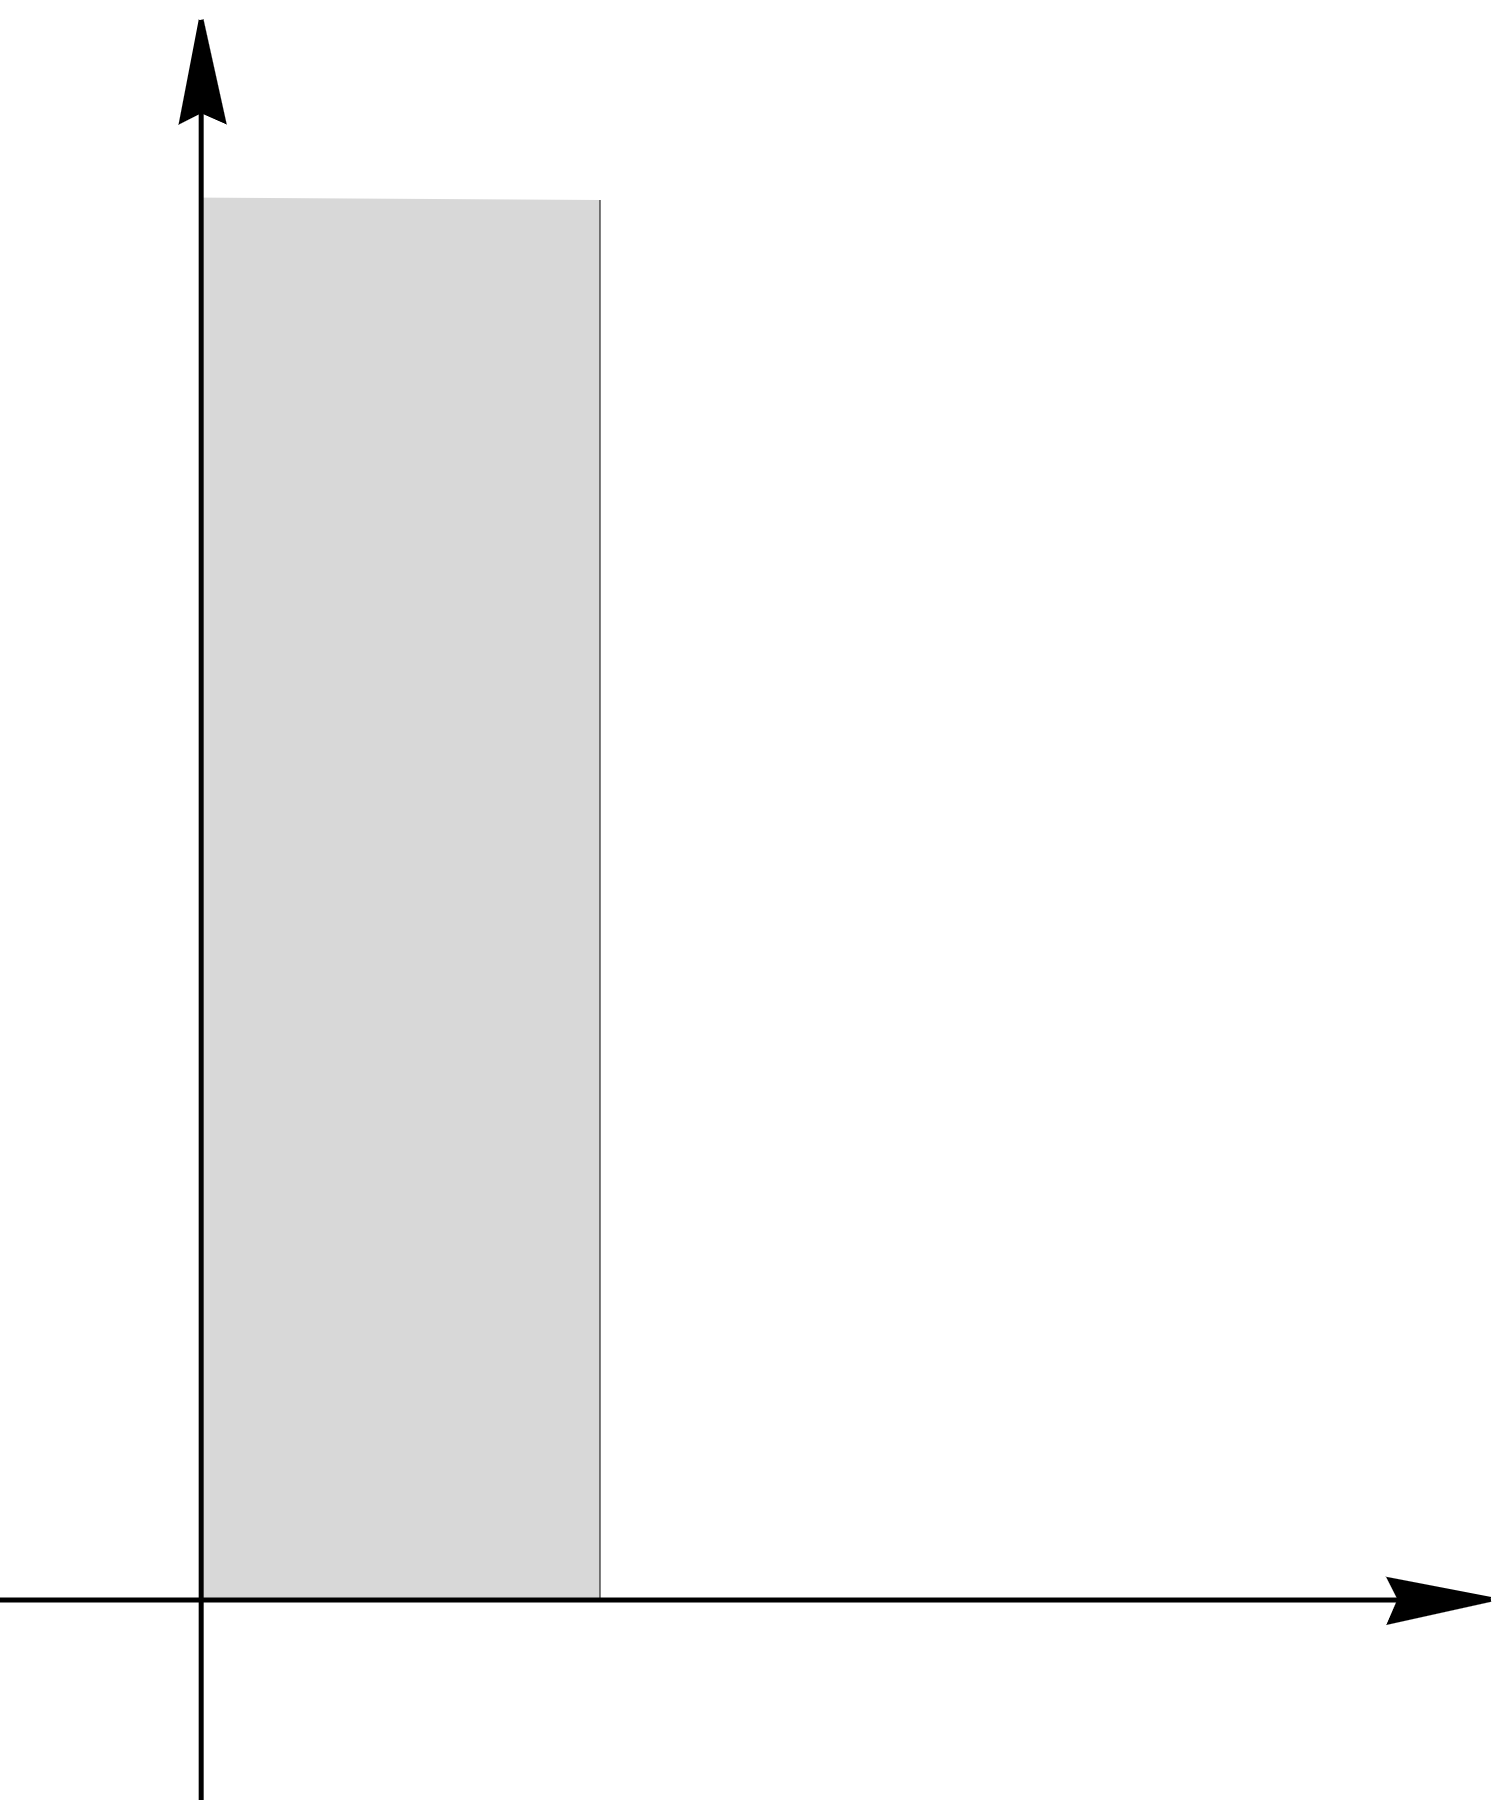
\includegraphics{pictures/heat_region.png}
        }};
        \node at (2.8, -3) {$z$};
        \node at (-1.9, 3.3) {$t$};
        \node at (-0.55, -3) {$L$};
        \node at (-1.4, -3) {$t = 0$};
        \node at (-0.1, -1.3) {$z = L$};
        \node at (-2.7, -1.3) {$z = 0$};
        \node at (-2.5, 0.2) {$\mathbf{n}_2$};
        \node at (-0.2, 0.2) {$\mathbf{n}_1$};
        \node at (-1.4, 0.1) {$R$};
        \node (1) at (-0.72, 0) {};
        \node (2) at (0.3,0) {};
        \draw[-Stealth] (1) -- (2);

        \node (3) at (-2.05, 0) {};
        \node (4) at (-3.05,0) {};
        \draw[-Stealth] (3) -- (4);
    \end{tikzpicture}
    \centering 
    \caption{The domain for the heat equation.} 
    \label{fig.heat_region} 
\end{figure}

There are three pieces of $\partial R$, 
\begin{equation}\label{eq.heat_boundary_3_pieces}
    \begin{split}
        &z=0, \quad t>0
        \\
        &z=L, \quad t>0
        \\
        &0<z<L, \quad t=0
    \end{split}
\end{equation}

On the first two parts of $\partial R$ corresponding to $z = 0,\, L$, we impose Robin boundary condition. On the last part corresponding to $t = 0$, we impose the Dirichlet boundary condition. Then we get the following system of equations,
\begin{equation}\label{eq.heat_and_boundary_1}
    \left\{\begin{aligned} 
        &u_t=K u_{z z}, && 0<z<L, \quad t>0, 
        \\ 
        &a(z, t) u+b(z, t) \mathbf{n} \cdot \nabla u=g(z, t),\quad && z=0,\, L, \quad t>0, 
        \\
        &u(z, 0)=f(z), && 0<z<L, \quad t=0.
    \end{aligned}\right.
\end{equation}
Here the choice of Dirichlet and Robin boundary condition comes from the physics of heat conduction. We will explain this in section \ref{sec.}.

\textbf{TODO: second order need one condition but first order need one}


Now we explain how to simplify the Robin boundary condition in \eqref{eq.heat_and_boundary_1}.

On $z = 0$, from figure \ref{fig.heat_region}, we know that the normal vector $\mathbf{n} = (-1, 0)$ and $\nabla u = (u_z, u_t)$, so we get $\mathbf{n}\cdot \nabla u = -u_z$. Therefore, $a(z, t) u+b(z, t) \mathbf{n} \cdot \nabla u=g(z, t)$ simplifies to 
\begin{equation}\label{eq.heat_and_boundary_2}
    a(0, t) u - b(0, t) u_z = g(0, t).
\end{equation}

On $z = L$, from figure \ref{fig.heat_region}, we know that the normal vector $\mathbf{n} = (1, 0)$ and $\nabla u = (u_z, u_t)$, so we get $\mathbf{n}\cdot \nabla u = u_z$. Therefore, $a(z, t) u+b(z, t) \mathbf{n} \cdot \nabla u=g(z, t)$ simplifies to 
\begin{equation}\label{eq.heat_and_boundary_3}
    a(L, t) u + b(L, t) u_z = g(L, t).
\end{equation}

We introduce new functions $a(t)$, $\widetilde{a}(t)$, $b(t)$, $\widetilde{b}(t)$, $g(t)$ and $\widetilde{g}(t)$ by the following equations
\begin{equation}\label{eq.heat_and_boundary_4}
    \begin{split}
        &a(t) = a(0, t),\quad b(t) = b(0, t),\quad g(t) = g(0, t)
        \\
        &\widetilde{a}(t) = a(L, t),\quad \widetilde{b}(t) = b(L, t),\quad \widetilde{g}(t) = g(L, t)
    \end{split}
\end{equation}

Then the Robin boundary conditions becomes
\begin{equation}\label{eq.heat_and_boundary_5}
    \begin{split}
        &a(t) u - b(t) u_z = g(t), \quad z = 0
        \\
        &\widetilde{a}(t) u + \widetilde{b}(t) u_z = \widetilde{g}(t), \quad z = L
    \end{split}
\end{equation}

The heat equation becomes
\begin{equation}\label{eq.heat_and_boundary_general}
    \left\{\begin{aligned} 
        &u_t=K u_{z z}, && 0<z<L, \quad t>0, 
        \\ 
        &a(t) u - b(t) u_z = g(t),\quad && z=0, \quad t>0, 
        \\ 
        &\widetilde{a}(t) u + \widetilde{b}(t) u_z = \widetilde{g}(t), && z=L, \quad t>0, 
        \\
        &u=f(z), && 0<z<L, \quad t=0.
    \end{aligned}\right.
\end{equation}

In order to make \eqref{eq.heat_and_boundary_general} solvable, we impose the homogeneous condition. 


\begin{definition}[Homogeneous] We say \eqref{eq.heat_and_boundary_general} is \underline{homogeneous} if 
    \begin{enumerate}
        \item $a(t)$, $\widetilde{a}(t)$, $b(t)$, $\widetilde{b}(t)$, $g(t)$ and $\widetilde{g}(t)$ are independent of $t$.
        \item $g(t) = \widetilde{g}(t) = 0$.
    \end{enumerate}
\end{definition}

With homogeneous assumption, \eqref{eq.heat_and_boundary_general} becomes
\begin{equation}\label{eq.heat_and_boundary_6}
    \left\{\begin{aligned} 
        &u_t=K u_{z z}, && 0<z<L, \quad t>0, 
        \\ 
        &a u - b u_z = 0,\quad && z=0, \quad t>0, 
        \\ 
        &\widetilde{a} u + \widetilde{b} u_z = 0, && z=L, \quad t>0, 
        \\
        &u=f(z), && 0<z<L, \quad t=0.
    \end{aligned}\right.
\end{equation}

To further simplify the above equation, we doing the change of variable 
\begin{equation}
    b\rightarrow bL,\quad \widetilde{b}\rightarrow \widetilde{b}L
\end{equation}
followed by the change of variable
\begin{equation}
    \begin{split}
        &a\rightarrow r\cos \alpha,\quad b\rightarrow r\sin \alpha,
        \\
        &\widetilde{a}\rightarrow r\cos \beta,\quad \widetilde{b}\rightarrow r\sin \beta.
    \end{split}
\end{equation}

Finally, the heat equation becomes
\begin{equation}\label{eq.heat_and_boundary}
    \left\{\begin{aligned} 
        &u_t=K u_{z z}, && 0<z<L, \quad t>0, 
        \\ 
        &u \cos \alpha-L u_z \sin \alpha=0,\quad && z=0, \quad t>0, 
        \\ 
        &u \cos \beta+L u_z \sin \beta=0, && z=L, \quad t>0, 
        \\
        &u=f(z), && 0<z<L, \quad t=0,
    \end{aligned}\right.
\end{equation}


\subsubsection{Separation of variable in heat equation}

Let us solve the heat equation in a simple case of $\alpha=\beta=0$ in \eqref{eq.heat_and_boundary}. The separated solution is written as $u(z, t)=\phi(z) T(t)$. Thus we obtain
$$
T^{\prime}(t)+\lambda K T(t)=0, \quad \phi^{\prime \prime}(z)+\lambda \phi(z)=0 .
$$

The boundary conditions are written as
$$
\phi(0)=\phi(L)=0 .
$$

We obtain
$$
T(t)=e^{-\lambda K t}, \quad \phi=A \sin (\sqrt{\lambda} z)+B \cos (\sqrt{\lambda} z), \quad \lambda>0 .
$$

By plugging $\phi=A \sin (\sqrt{\lambda} z)+B \cos (\sqrt{\lambda} z)$ into the boundary conditions, we find that $B=0$ and $\sqrt{\lambda} L = n\pi$ where $n$ is an integer. Therefore we obtain
$$
\phi(z)=\phi_n(z)=\sin \left(\sqrt{\lambda_n} z\right), \quad \lambda_n=\left(\frac{n \pi}{L}\right)^2, \quad n=1,2, \ldots,
$$
where we set the arbitrary constant in $\phi_n(z)$ to be $1$ (recall we will take a superposition). Thus the separated solutions are obtained as
$$
u(z, t)=\phi_n(z) e^{-\lambda_n K t}, \quad n=1,2, \ldots
$$

If no initial condition $u(z, 0) = f(z)$ is given, the above separated solutions are the solutions to the problem. However, they do not satisfies $u(z, 0) = f(z)$.
Let us consider the linear combination of separated solution and match with the initial condition.

The linear combination is 
$$
u(z, t)=\sum_{n=1}^{\infty} C_n \phi_n(z) e^{-\lambda_n K t},
$$
where $C_n$ are constants. 

By $u(z, 0) = f(z)$, we know that 

$$
f(z) = u(z, 0) = \sum_{n=1}^{\infty} C_n \phi_n(z) = \sum_{n=1}^{\infty} C_n \sin \frac{n\pi z}{L}.
$$

From this we know that $C_n$ is the $B_n$ coefficients of the Fourier sine series. We thus obtain
$$
u(z, t)=\sum_{n=1}^{\infty} B_n \phi_n(z) e^{-\lambda_n K t}, \quad 0<z<L, \quad t>0 .
$$
$$
B_n=\frac{2}{L} \int_0^L f(x) \sin \frac{n \pi x}{L} d x.
$$

\begin{example}[]
The heat equation $u_t=K u_{z z}$ for $0<z<L, t>0$ with $u(0, t)=u(L, t)=0$ and $u(z, 0)=1$ is solved as
$$
u(z, t)=\sum_{n=1}^{\infty} B_n \sin \frac{n \pi z}{L} e^{-(n \pi / L)^2 K t},
$$
where  
$$
B_n=\frac{2}{\pi} \frac{1-(-1)^n}{n} .
$$

Here as mentioned above, $B_n$ can be directly computed as coefficients of the Fourier sine series of $f(z) = 1$
\end{example}

\subsubsection{Some linear algebra}


\subsection{The Sturm-Liouville eigenvalue problem}

\subsubsection{Orthogonal functions}

\begin{definition}[Inner product] We extend dot product $\varphi \cdot \psi$ and define \underline{inner product} as
\begin{equation}\label{eq.inner_product}
    \langle\varphi, \psi\rangle=\int_a^b \varphi(x) \psi(x) d x .
\end{equation}
    
Sometimes the inner product is defined as follows. We can have a \underline{weight function} $\rho(x)$, and the weighted inner product is given by
\begin{equation}\label{eq.inner_product_weight}
    \langle\varphi, \psi\rangle_\rho=\int_a^b \varphi(x) \psi(x) \rho(x) d x
\end{equation}
where $\rho(x)>0$ is a weight function. 

For complex functions, we can write the \underline{complex inner product} as
\begin{equation}\label{eq.inner_product_complex}
    \langle\varphi, \psi\rangle=\int_a^b \varphi(x) \bar{\psi}(x) \rho(x) d x .
\end{equation}
Here $\bar{\psi}$ is the complex conjugate of $\psi$ $(\bar{\psi}(x)=f(x)-i g(x)$ when $\psi=f+i g)$.
    
\end{definition}

\begin{definition}[Orthogonality]
Two functions $\varphi, \psi$ are said to be \underline{orthogonal} on $[a, b]$ if $\langle\varphi, \psi\rangle=0$.    
\end{definition}

\begin{example}[]
    The functions $\varphi(x)=\sin x$ and $\psi(x)=\cos x$ are orthogonal on $[0, \pi]$.
\end{example}
\begin{example}[]
    The set of functions $\sin x, \sin 2 x, \ldots, \sin N x$ is orthogonal on $[0, \pi]$.
\end{example}
\begin{example}[]
    Which of the following pairs of functions are orthogonal on the interval $0 \leq x \leq 1$ ?
$$
\varphi_1=\sin 2 \pi x, \quad \varphi_2=x, \quad \varphi_3=\cos 2 \pi x, \quad \varphi_4=1 .
$$
$\left\langle\varphi_1, \varphi_3\right\rangle=0,\left\langle\varphi_1, \varphi_4\right\rangle=0,\left\langle\varphi_2, \varphi_3\right\rangle=0,\left\langle\varphi_3, \varphi_4\right\rangle=0$. All others are nonzero. Therefore the pairs $\left(\varphi_1, \varphi_3\right),\left(\varphi_1, \varphi_4\right),\left(\varphi_2, \varphi_3\right)$, and $\left(\varphi_3, \varphi_4\right)$ are orthogonal.
\end{example}

\begin{definition}[Norm]
As follows we define \underline{norm}, which is the ``length'' of a function.
$$
\|\varphi\|=\|\varphi\|_{L^2(a, b)}=\sqrt{\langle\varphi, \varphi\rangle} .
$$
We note that the norm is always nonnegative. The norm $\|\varphi-\psi\|$ is the distance between two functions $\varphi$ and $\psi$.
\end{definition}

\begin{definition}[Projection]
    Let $\left(\varphi_1, \ldots, \varphi_N\right)$ be a set of orthogonal functions with $\left\|\varphi_i\right\| \neq 0$. Let $f(x)$ be a function. Then $\hat{c}_1 \varphi_1+\cdots+\hat{c}_N \varphi_N$ with $\hat{c}_i=$ $\left\langle f, \varphi_i\right\rangle /\left\|\varphi_i\right\|^2$ is the projection of $f$ onto $\left(\varphi_1, \ldots, \varphi_N\right) . \hat{c}_i$ is called the $i$ th Fourier coefficient of $f$. 

    \textbf{TODO: revise this}
\end{definition}


Note that the minimum of $\left\|f-\left(c_1 \varphi_1+\cdots+c_N \varphi_N\right)\right\|$ is achieved when $c_i=\hat{c}_i$.
    
\begin{example}[]
    Find the projection of $f(x)=1$ onto $\left(\varphi_1, \varphi_2\right)=(\sin x, \sin 2 x)$ on the interval $0 \leq x \leq \pi$. By $\left\langle f, \varphi_1\right\rangle=2,\left\langle f, \varphi_2\right\rangle=0$, and $\left\|\varphi_1\right\|^2=\left\|\varphi_2\right\|^2=\frac{\pi}{2}$, we obtain $\frac{4}{\pi} \sin x$.   
\end{example}

\begin{definition}[Orthonormal]
    The functions $\left(\varphi_1, \ldots, \varphi_N\right)$ are orthonormal if $\left\langle\varphi_i, \varphi_j\right\rangle=$ $\delta_{i j}$. Here $\delta_{i j}$ is the Kronecker delta $(\delta_{i j}=0$ if $i \neq j$ and $=1$ if $i=j)$.
\end{definition}

\subsubsection{The Sturm-Liouville eigenvalue problem}

\subsubsection{Convergence of orthogonal series}

\subsection{The heat equation}

\subsubsection{Physics of heat conduction}

\subsubsection{The homogeneous case}

\subsubsection{The non-homogeneous case}

\subsection{The wave equation}

\subsubsection{Physics of string vibration}

\subsubsection{The homogeneous case}

\subsubsection{The non-homogeneous case}


\subsection{The Laplace's equation}

\subsubsection{Physics of static electricity}

\subsubsection{The homogeneous case}

\subsubsection{The non-homogeneous case}